% This is the Duke University Statistical Science LaTeX thesis template.
% It has been adapted from the Reed College LaTeX thesis template. The
% adaptation was done by Mine Cetinkaya-Rundel (MCR). Some of the comments
% that are specific to Reed College have been removed.
%
% Most of the work on the original Reed College document class and template
% was done by Sam Noble (SN). Later comments etc. by Ben Salzberg (BTS).
% Additional restructuring and APA support by Jess Youngberg (JY).
%
% See https://www.reed.edu/cis/help/latex/ for help. There are a
% great bunch of help pages there, with notes on
% getting started, bibtex, etc. Go there and read it if you're not
% already familiar with LaTeX.
%
% Any line that starts with a percent symbol is a comment.
% They won't show up in the document, and are useful for notes
% to yourself and explaining commands.
% Commenting also removes a line from the document;
% very handy for troubleshooting problems. -BTS

%%
%% Preamble
%%
% \documentclass{<something>} must begin each LaTeX document
\documentclass[12pt,twoside]{dukestatscithesis}
% Packages are extensions to the basic LaTeX functions. Whatever you
% want to typeset, there is probably a package out there for it.
% Chemistry (chemtex), screenplays, you name it.
% Check out CTAN to see: http://www.ctan.org/
%%
\usepackage{graphicx,latexsym}
\usepackage{amsmath}
\usepackage{amssymb,amsthm}
\usepackage{longtable,booktabs,setspace}
\usepackage{chemarr} %% Useful for one reaction arrow, useless if you're not a chem major
\usepackage[hyphens]{url}
% Added by CII
\usepackage{hyperref}
\usepackage{lmodern}
\usepackage{float}
\floatplacement{figure}{H}
% End of CII addition
\usepackage{rotating}

% Next line commented out by CII
%%% \usepackage{natbib}
% Comment out the natbib line above and uncomment the following two lines to use the new
% biblatex-chicago style, for Chicago A. Also make some changes at the end where the
% bibliography is included.
%\usepackage{biblatex-chicago}
%\bibliography{thesis}


% Added by CII (Thanks, Hadley!)
% Use ref for internal links
\renewcommand{\hyperref}[2][???]{\autoref{#1}}
\def\chapterautorefname{Chapter}
\def\sectionautorefname{Section}
\def\subsectionautorefname{Subsection}
% End of CII addition

% Added by CII
\usepackage{caption}
\captionsetup{width=5in}
% End of CII addition

% \usepackage{times} % other fonts are available like times, bookman, charter, palatino


% To pass between YAML and LaTeX the dollar signs are added by CII
\title{}
\author{}
% The month and year that you submit your FINAL draft TO THE LIBRARY (May or December)
\date{}
\advisor{}
\institution{}
\degree{}
\committeememberone{}
\committeemembertwo{}
\dus{}
%If you have two advisors for some reason, you can use the following
% Uncommented out by CII
% End of CII addition

%%% Remember to use the correct department!
\department{}

% Added by CII
%%% Copied from knitr
%% maxwidth is the original width if it's less than linewidth
%% otherwise use linewidth (to make sure the graphics do not exceed the margin)
\makeatletter
\def\maxwidth{ %
  \ifdim\Gin@nat@width>\linewidth
    \linewidth
  \else
    \Gin@nat@width
  \fi
}
\makeatother

\renewcommand{\contentsname}{Table of Contents}
% End of CII addition

\setlength{\parskip}{0pt}

% Added by CII

\providecommand{\tightlist}{%
  \setlength{\itemsep}{0pt}\setlength{\parskip}{0pt}}

\Acknowledgements{

}

\Dedication{

}

\Preface{

}

\Abstract{

}

% End of CII addition
%%
%% End Preamble
%%
%

\usepackage{amsthm}
\newtheorem{theorem}{Theorem}[chapter]
\newtheorem{lemma}{Lemma}[chapter]
\theoremstyle{definition}
\newtheorem{definition}{Definition}[chapter]
\newtheorem{corollary}{Corollary}[chapter]
\newtheorem{proposition}{Proposition}[chapter]
\theoremstyle{definition}
\newtheorem{example}{Example}[chapter]
\theoremstyle{definition}
\newtheorem{exercise}{Exercise}[chapter]
\theoremstyle{remark}
\newtheorem*{remark}{Remark}
\newtheorem*{solution}{Solution}
\begin{document}

% Everything below added by CII

\frontmatter % this stuff will be roman-numbered
\pagestyle{empty} % this removes page numbers from the frontmatter



  \hypersetup{linkcolor=black}
  \setcounter{tocdepth}{2}
  \tableofcontents





\mainmatter % here the regular arabic numbering starts
\pagestyle{fancyplain} % turns page numbering back on

\chapter*{Preliminary Content}\label{preliminary-content}
\addcontentsline{toc}{chapter}{Preliminary Content}

\section*{Acknowledgements}\label{acknowledgements}
\addcontentsline{toc}{section}{Acknowledgements}

I thank my advisor, Professor Peter Hoff, and the Director of
Undergraduate Studies, Professor Mine Cetinkaya-Rundel, for their
guidance in this project. I also thank Duke University's Statistics
Department and Office of Information Technology, especially my dataset
contact at OIT, Eric Hope, for making this project possible. Most of all
I thank my parents for their continued unwavering support in all my
endeavors.

The goal of this project is to identify novel methods for detecting
anomalies in network IP data. The space is represented as a
3-dimensional tensor of the continuous features (source bytes,
destination bytes, source packets, destination packets) divided by their
respective source port and destination port combinations. This project
implements and assesses the validity of principal component analysis and
matrix completion via singular value decomposition (more methods
pending) in determining anomalous entries in the tensor.

\chapter{Introduction}\label{introduction}

\section{Anomaly Detection}\label{anomaly-detection}

Anomaly detection is used to identify unusual patterns or observations
that do not conform to expected behavior in a dataset. Anomalies can be
broadly categorized into three categories:

Point anomalies: A single instance of data is anomalous if it's too far
off from the rest. For example detecting credit card fraud based on a
single spending spree that represents the credit card being stolen and
used.

Contextual anomalies: The abnormality is context specific. This type of
anomaly is common in time-series data. For instance, high spending on
food and gifts every day during the holiday season is normal, but may be
considered unusual otherwise.

Collective anomalies: A set of data observations that when collectively
assessed helps in detecting anomalies. For instance, repeated pings from
a certain IP address to a port connection on a hosted network may be
classified as a port scanner, which often preludes a network attack.

\section{Network Attacks}\label{network-attacks}

Network security is becoming increasingly relevant as the flow of data,
bandwith of transactions, and user dependency on hosted networks
increase. As entire networks grow in nodes and complexity, attackers
gain easier entry points of access to the network. The most benign of
attackers attempt to shutdown networks (e.g.~causing a website to
shutdown with repeated pings to its server), while more malicious
attempts involve hijacking the server to publish the attacker's own
content or stealing unsecured data from the server, thus compromising
the privacy of the network's users.

Attackers follow a specific three step strategy when gathering
intelligence on a network, the most important component of which is
scanning. Network scanning is a procedure for identifying active hosts
on a network, the attacker uses it to find information about the
specific IP addresses that can be accessed over the Internet, their
target's operating systems, system architecture, and the services
running on each node/computer in the network. Scanning procedures, such
as ping sweeps and port scans, return information about which IP
addresses map to live hosts that are active on the Internet and what
services they offer. Another scanning method, inverse mapping, returns
information about what IP addresses do not map to live hosts; this
enables an attacker to make assumptions about viable addresses.

All three of these scanning methods leave digital signatures in the
networks they evaluate because they apply specific pings that are then
stored in the network logs. Most scanners use a specific combination of
bytes, packets, flags (in TCP protocol), and ports in a sequence of
pings to a network. Identifying a scanner's often many IP addresses from
the set of pings available in the network's logs is thus an anomaly
detection problem. In particular, because the data is unlabeled, meaning
it is unclear which observations are actually scanners and which are
just standard user behavior, unsupervised approaches are necessary for
tackling the problem.

This particular dataset is from Duke University's Office of Information
Technology (OIT), and it covers all observations in their network
traffic during a five minute period in February 2017.

\subsection{Status Quo Solution}\label{status-quo-solution}

OIT's current solution for detecting scanners relies on specific domain
knowledge gathered from diagnostics programs and data analysis completed
on previous data. They prevent scanners by blocking IP addresses that
fit certain rules they have constructed to run on every network
transaction as it occurs. The specific checks in these rules are private
for security reasons, but they belong to the nature of evaluating the
size of transactions, repeated connections between particular ports,
many pings from the same address, and combinations of these particular
behaviors.

While this solution presents a methodical way for banning IP addresses
and its method of rule checking is essentially removing what OIT
considers outliers for network transactions-any observation that does
not fit within the constraints specified by the rules is classified as
an outleir and its source IP is blocked-it is inflexible, prone to
detecting false negatives, and fails to detect observations that may be
within the parameter constraints of the rules but are anomalous with
respect to other parameters or parameter constraints.

\section{Network Dataset}\label{network-dataset}

\subsection{Features}\label{features}

The networks dataset contains 13 features, 8 categorical and 5
continuous, and the observations are unlabeled (not specified whether
they are considered a scanner). The 13 features are:

\textbf{Continuous:}
\begin{itemize}
\tightlist
\item
  StartTime (Start Time): the time when the observation is logged
\item
  SrcBytes (Source Bytes): the total number of bytes sent in the
  observation
\item
  SrcPkts (Source Packets): the number of packets sent in the
  observation
\item
  DstBytes (Destination Bytes): the total number of bytes received in
  the observation
\item
  DstPkts (Destination Packets): the number of packets received in the
  observation Note, the destination packets and bytes features do not
  have the same values as their source counterparts because the
  connections are compressed and decompressed into different forms and
  byte sizes when sent. For instance, it is possible for the number of
  destination packets to be larger than source packets. It is also
  possible for information to be lost during the connection.
\end{itemize}
\textbf{Categorical:}
\begin{itemize}
\tightlist
\item
  Flgs (connection flag): flow state flags seen in transaction between
  the two addresses
\item
  Proto (network protocol): specifies the rules used for information
  exchange via network addresses. Transmission Control Protocol (TCP)
  uses a set of rules to exchange messages with other Internet points at
  the information packet level, and Internet Protocol (IP) uses a set of
  rules to send and receive messages at the Internet address level.
\item
  SrcAddr (Source Address): the IP address of the connection's source
\item
  DstAddr (Destination Address): the IP address of the connection's
  destination
\item
  Sport (Source Port): the network port number of the connection's
  source. A port numbers identifies the specific process to which a
  network message is forwarded when it arrives at a server.
\item
  Dport (Destination Port): the network port number of the connection's
  destination
\item
  Dir (direction): the direction of the connection
\item
  State (connection state): a categorical assessment of the current
  phase in the transaction when the timestamp is recorded
\end{itemize}
Note, the addresses have been anonymized for security reasons.

\subsection{Argus}\label{argus}

Argus is the open source network security tool applied to network
transactions that collects the data for the features. The Argus wiki and
the OIT manual provides key insights into the structure and nature of
the data. Specifically, the sessions are clustered together by address,
so the pytes and packets values are accumulative over a set duration and
each session has its own start time but does not have a tracked end
time. There exist 2-4 million connections on average every 5 minutes.
Furthermore the protocol in this dataset is always gathered from TCP
protocol and the direction will always be to the right (i.e.~Source to
Destination). This information supports dropping proto, StartTime, and
Direction from the dataset for future analysis because they do not
present any information regarding whether an observation can be
considered an anomaly. Furthermore, the State feature may not be
reliable because Argus occasionally resets the state data statistics
during monitoring.

\chapter{Modeling Port Relationships}\label{modeling-port-relationships}

\section{Motivation}\label{motivation}

Exploratory data analysis signaled that there may exist trends between
different port combinations. For instance, a particular source and
destination port may frequently contain large byte transactions in their
connections. Devising a systematic way to identify these combinations
may present outliers that can be further investigated for scanner
behavior.

Beginning the investigation requires the creation of a 2-dimensional
matrix of the most common source and destination port combinations. Each
cell in this matrix is of variable length and holds all of the data
observations involving that particular source and destination port
pairing. Following the creation of this matrix, principal component
analysis may be applied to the combinations present in each cell to
investigate the behavior of that specific connection.

\section{Principal Component
Analysis}\label{principal-component-analysis}

Principal component analysis represents data in terms of its principal
components rather than relying on traditional Cartesian axes. Principal
components contain the underlying structure in data by representing the
directions that contain the most variance. Each successive principal
component is orthoganol to the previous, so the resulting vectors yields
an uncorrelated orthogonal basis set. Because PCA is sensitive to
relative scaling of variables, a normal scores transformation is applied
before the algorithm is run.

\subsection{Application}\label{application}

In this problem, Principal Component Anaylsis is applied to each
source-destination port grouping of observed data to understand the
underlying structure of the data partition's continuous features: source
bytes and packets and destination bytes and packets. In particular the
amount of variance explained by the generated principal components and
their relative directions will signal whether specific trends in
connection behavior occur at certain ports, and whether the size of each
of the continuous features affects port behavior as well as the other
features.

\section{Implementation}\label{implementation}

\subsection{Ports Combination
Matrix/Tensor}\label{ports-combination-matrixtensor}
\begin{Shaded}
\begin{Highlighting}[]
\CommentTok{#set counts}
\NormalTok{s_num =}\StringTok{ }\DecValTok{25}
\NormalTok{d_num =}\StringTok{ }\DecValTok{25}
\NormalTok{combo_num =}\StringTok{ }\DecValTok{20}

\CommentTok{#get top sport and dport values}
\NormalTok{Sport_table =}\StringTok{ }\KeywordTok{table}\NormalTok{(Sport)}
\NormalTok{Sport_table =}\StringTok{ }\KeywordTok{as.data.frame}\NormalTok{(Sport_table)}
\NormalTok{Sport_table =}\StringTok{ }\NormalTok{Sport_table[}\KeywordTok{order}\NormalTok{(-Sport_table$Freq),]}
\NormalTok{top_Sport =}\StringTok{ }\NormalTok{(}\KeywordTok{head}\NormalTok{(Sport_table$Sport, s_num))}

\NormalTok{Dport_table =}\StringTok{ }\KeywordTok{table}\NormalTok{(Dport)}
\NormalTok{Dport_table =}\StringTok{ }\KeywordTok{as.data.frame}\NormalTok{(Dport_table)}
\NormalTok{Dport_table =}\StringTok{ }\NormalTok{Dport_table[}\KeywordTok{order}\NormalTok{(-Dport_table$Freq),]}
\NormalTok{top_Dport =}\StringTok{ }\NormalTok{(}\KeywordTok{head}\NormalTok{(Dport_table$Dport, d_num))}

\CommentTok{#subset data for the combinations}
\NormalTok{argus_maxes =}\StringTok{ }\NormalTok{argus[}\KeywordTok{is.element}\NormalTok{(Sport, top_Sport) &}\StringTok{ }\KeywordTok{is.element}\NormalTok{(Dport, top_Dport), ]}
\NormalTok{argus_maxes =}\StringTok{ }\KeywordTok{transform}\NormalTok{(argus_maxes,}
                        \DataTypeTok{Sport =} \KeywordTok{as.numeric}\NormalTok{(}\KeywordTok{as.character}\NormalTok{(Sport)),}
                        \DataTypeTok{Dport =} \KeywordTok{as.numeric}\NormalTok{(}\KeywordTok{as.character}\NormalTok{(Dport)))}
\NormalTok{max_combinations =}\StringTok{ }\KeywordTok{as.data.frame}\NormalTok{(}\KeywordTok{table}\NormalTok{(argus_maxes$Sport, argus_maxes$Dport))}

\NormalTok{top_combinations =}\StringTok{ }\KeywordTok{head}\NormalTok{(max_combinations[}\KeywordTok{order}\NormalTok{(-max_combinations$Freq),], combo_num)}
\NormalTok{top_combinations$Sport =}\StringTok{ }\NormalTok{top_combinations$Var1}
\NormalTok{top_combinations$Dport =}\StringTok{ }\NormalTok{top_combinations$Var2}
\NormalTok{top_combinations$Var1 =}\StringTok{ }\OtherTok{NULL}
\NormalTok{top_combinations$Var2 =}\StringTok{ }\OtherTok{NULL}
\NormalTok{top_combinations =}\StringTok{ }\KeywordTok{transform}\NormalTok{(top_combinations,}
                             \DataTypeTok{Sport =} \KeywordTok{as.numeric}\NormalTok{(}\KeywordTok{as.character}\NormalTok{(Sport)),}
                             \DataTypeTok{Dport =} \KeywordTok{as.numeric}\NormalTok{(}\KeywordTok{as.character}\NormalTok{(Dport)))}

\CommentTok{#generate the combinations matrix of ports}
\NormalTok{extract_intersection =}\StringTok{ }\NormalTok{function(sport, dport)\{}
  \NormalTok{argus_subset =}\StringTok{ }\NormalTok{argus[Sport ==}\StringTok{ }\NormalTok{sport &}\StringTok{ }\NormalTok{Dport ==}\StringTok{ }\NormalTok{dport,]}
  \KeywordTok{return} \NormalTok{(argus_subset)}
\NormalTok{\}}
\NormalTok{generate_combinations_matrix =}\StringTok{ }\NormalTok{function(top_combinations)\{}
  \NormalTok{n =}\StringTok{ }\KeywordTok{dim}\NormalTok{(top_combinations)[}\DecValTok{1}\NormalTok{]}
  \NormalTok{combinations =}\StringTok{ }\KeywordTok{c}\NormalTok{()}
  \NormalTok{for (i in }\DecValTok{1}\NormalTok{:n)\{}
    \NormalTok{sport =}\StringTok{ }\KeywordTok{as.numeric}\NormalTok{(top_combinations[i,]$Sport)}
    \NormalTok{dport =}\StringTok{ }\KeywordTok{as.numeric}\NormalTok{(top_combinations[i,]$Dport)}
    \NormalTok{combo =}\StringTok{ }\KeywordTok{extract_intersection}\NormalTok{(sport, dport)}
    \NormalTok{combinations =}\StringTok{ }\KeywordTok{c}\NormalTok{(combinations, }\KeywordTok{list}\NormalTok{(combo))}
  \NormalTok{\}}
  \KeywordTok{return} \NormalTok{(combinations)}
\NormalTok{\}}
\NormalTok{combinations =}\StringTok{ }\KeywordTok{generate_combinations_matrix}\NormalTok{(top_combinations)}
\end{Highlighting}
\end{Shaded}
\subsection{Investigating
Combinations}\label{investigating-combinations}
\begin{Shaded}
\begin{Highlighting}[]
\CommentTok{#principal component analysis and visualizing results}
\NormalTok{pca_analysis =}\StringTok{ }\NormalTok{function(SrcBytes, SrcPkts, DstBytes, DstPkts)\{}
  \NormalTok{pca_cont_vars =}\StringTok{ }\KeywordTok{cbind}\NormalTok{(SrcBytes, SrcPkts, DstBytes, DstPkts)}
  \NormalTok{pca =}\StringTok{ }\KeywordTok{prcomp}\NormalTok{(pca_cont_vars, }\DataTypeTok{center =} \OtherTok{TRUE}\NormalTok{, }\DataTypeTok{scale. =} \OtherTok{TRUE}\NormalTok{)}
  \KeywordTok{print}\NormalTok{(pca$rotation)}
  \KeywordTok{print}\NormalTok{((}\KeywordTok{summary}\NormalTok{(pca)))}
  \CommentTok{#screeplot(pca, type="lines",col=3)}
  \NormalTok{g =}\StringTok{ }\KeywordTok{ggbiplot}\NormalTok{(pca, }\DataTypeTok{obs.scale =} \DecValTok{1}\NormalTok{, }\DataTypeTok{var.scale =} \DecValTok{1}\NormalTok{,}
                \DataTypeTok{ellipse =} \OtherTok{TRUE}\NormalTok{,}
                \DataTypeTok{circle =} \OtherTok{TRUE}\NormalTok{)}
  \NormalTok{g =}\StringTok{ }\NormalTok{g +}\StringTok{ }\KeywordTok{scale_color_discrete}\NormalTok{(}\DataTypeTok{name =} \StringTok{''}\NormalTok{)}
  \NormalTok{g =}\StringTok{ }\NormalTok{g +}\StringTok{ }\KeywordTok{theme}\NormalTok{(}\DataTypeTok{legend.direction =} \StringTok{'horizontal'}\NormalTok{,}
                 \DataTypeTok{legend.position =} \StringTok{'top'}\NormalTok{)}
  \KeywordTok{print}\NormalTok{(g)}
  \KeywordTok{return}\NormalTok{(pca$rotation)}
\NormalTok{\}}
\CommentTok{#apply pca to the data partitions on the top 10 port combinations }
\NormalTok{combo_num =}\StringTok{ }\DecValTok{10}
\NormalTok{for (i in }\DecValTok{1}\NormalTok{:combo_num)\{}
  \NormalTok{combo_table =}\StringTok{ }\NormalTok{combinations[i]}
  \NormalTok{combo_table =}\StringTok{ }\KeywordTok{transform}\NormalTok{(combo_table,}
                          \DataTypeTok{SrcBytes =} \KeywordTok{as.numeric}\NormalTok{(SrcBytes),}
                          \DataTypeTok{SrcPkts =} \KeywordTok{as.numeric}\NormalTok{(SrcPkts),}
                          \DataTypeTok{DstBytes =} \KeywordTok{as.numeric}\NormalTok{(DstBytes),}
                          \DataTypeTok{DstPkts =} \KeywordTok{as.numeric}\NormalTok{(DstPkts))}
  \KeywordTok{cat}\NormalTok{(}\StringTok{"Sport:"}\NormalTok{, combo_table$Sport[}\DecValTok{1}\NormalTok{],}\StringTok{"}\CharTok{\textbackslash{}t}\StringTok{"}\NormalTok{)}
  \KeywordTok{cat}\NormalTok{(}\StringTok{"Dport:"}\NormalTok{, combo_table$Dport[}\DecValTok{1}\NormalTok{],}\StringTok{"}\CharTok{\textbackslash{}n}\StringTok{"}\NormalTok{)}
  \NormalTok{SrcBytes_norm =}\StringTok{  }\KeywordTok{nscore}\NormalTok{(combo_table$SrcBytes)$nscore}
  \NormalTok{SrcPkts_norm =}\StringTok{  }\KeywordTok{nscore}\NormalTok{(combo_table$SrcPkts)$nscore}
  \NormalTok{DstBytes_norm =}\StringTok{  }\KeywordTok{nscore}\NormalTok{(combo_table$DstBytes)$nscore}
  \NormalTok{DstPkts_norm =}\StringTok{  }\KeywordTok{nscore}\NormalTok{(combo_table$DstPkts)$nscore}
  \KeywordTok{pca_analysis}\NormalTok{(SrcBytes_norm, SrcPkts_norm, DstBytes_norm, DstPkts_norm)}
\NormalTok{\}}
\end{Highlighting}
\end{Shaded}
\begin{verbatim}
Sport: 32416    Dport: 9163 
               PC1        PC2        PC3          PC4
SrcBytes 0.4113308 -0.7246604 -0.5528760  0.001575730
SrcPkts  0.5054262 -0.3234250  0.7999554  0.003459252
DstBytes 0.5357591  0.4327433 -0.1665939  0.705649994
DstPkts  0.5369483  0.4277813 -0.1632360 -0.708550377
Importance of components:
                          PC1    PC2     PC3     PC4
Standard deviation     1.7118 0.8991 0.51065 0.02309
Proportion of Variance 0.7326 0.2021 0.06519 0.00013
Cumulative Proportion  0.7326 0.9347 0.99987 1.00000
\end{verbatim}
\includegraphics{thesis_files/figure-latex/unnamed-chunk-6-1.pdf}
\begin{verbatim}
Sport: 4145     Dport: 9119 
               PC1        PC2        PC3          PC4
SrcBytes 0.4333309  0.8902089 -0.1405308  0.001886624
SrcPkts  0.5213529 -0.1206221  0.8439979  0.036180840
DstBytes 0.5190742 -0.3165495 -0.3953966  0.688490995
DstPkts  0.5205549 -0.3045896 -0.3340362 -0.724339380
Importance of components:
                         PC1    PC2     PC3     PC4
Standard deviation     1.875 0.6538 0.23124 0.05551
Proportion of Variance 0.879 0.1069 0.01337 0.00077
Cumulative Proportion  0.879 0.9859 0.99923 1.00000
\end{verbatim}
\includegraphics{thesis_files/figure-latex/unnamed-chunk-6-2.pdf}
\begin{verbatim}
Sport: 19239    Dport: 9153 
               PC1        PC2        PC3          PC4
SrcBytes 0.4400190  0.8125062 -0.3823817 -0.001104223
SrcPkts  0.5189497  0.1174251  0.8466938 -0.003489750
DstBytes 0.5179403 -0.4057384 -0.2640886 -0.705245607
DstPkts  0.5184712 -0.4017728 -0.2591352  0.708953621
Importance of components:
                          PC1    PC2     PC3     PC4
Standard deviation     1.8418 0.7037 0.33316 0.03695
Proportion of Variance 0.8481 0.1238 0.02775 0.00034
Cumulative Proportion  0.8481 0.9719 0.99966 1.00000
\end{verbatim}
\includegraphics{thesis_files/figure-latex/unnamed-chunk-6-3.pdf}
\begin{verbatim}
Sport: 4243     Dport: 27 
               PC1        PC2        PC3          PC4
SrcBytes 0.3986539  0.8262979 -0.3978739  0.001762539
SrcPkts  0.5268775  0.1487193  0.8367993  0.007045781
DstBytes 0.5300998 -0.3876467 -0.2708012  0.703840168
DstPkts  0.5314785 -0.3805842 -0.2610173 -0.710321243
Importance of components:
                          PC1    PC2     PC3     PC4
Standard deviation     1.7727 0.8343 0.40033 0.03406
Proportion of Variance 0.7856 0.1740 0.04007 0.00029
Cumulative Proportion  0.7856 0.9596 0.99971 1.00000
\end{verbatim}
\includegraphics{thesis_files/figure-latex/unnamed-chunk-6-4.pdf}
\begin{verbatim}
Sport: 4243     Dport: 10290 
                PC1         PC2        PC3          PC4
SrcBytes -0.4146349  0.86007431 -0.2972268 -0.002501828
SrcPkts  -0.5225073  0.04229265  0.8514240 -0.016572825
DstBytes -0.5257892 -0.36545098 -0.3181251 -0.699133556
DstPkts  -0.5278350 -0.35345310 -0.2924547  0.714794623
Importance of components:
                          PC1    PC2     PC3     PC4
Standard deviation     1.8125 0.7560 0.37528 0.05022
Proportion of Variance 0.8213 0.1429 0.03521 0.00063
Cumulative Proportion  0.8213 0.9642 0.99937 1.00000
\end{verbatim}
\includegraphics{thesis_files/figure-latex/unnamed-chunk-6-5.pdf}
\begin{verbatim}
Sport: 4243     Dport: 26 
               PC1         PC2        PC3          PC4
SrcBytes 0.4320683  0.87332152 -0.2249932  0.002131619
SrcPkts  0.5202875 -0.03769203  0.8529953  0.016712305
DstBytes 0.5202102 -0.34831316 -0.3463831  0.698625865
DstPkts  0.5215355 -0.33847715 -0.3190547 -0.715288791
Importance of components:
                          PC1    PC2     PC3    PC4
Standard deviation     1.8559 0.6797 0.30326 0.0398
Proportion of Variance 0.8611 0.1155 0.02299 0.0004
Cumulative Proportion  0.8611 0.9766 0.99960 1.0000
\end{verbatim}
\includegraphics{thesis_files/figure-latex/unnamed-chunk-6-6.pdf}
\begin{verbatim}
Sport: 4243     Dport: 25 
               PC1        PC2        PC3           PC4
SrcBytes 0.4278586  0.8931432 -0.1386797 -0.0005117289
SrcPkts  0.5214493 -0.1186010  0.8449812 -0.0055942005
DstBytes 0.5218835 -0.3078511 -0.3699338 -0.7042828114
DstPkts  0.5221736 -0.3057071 -0.3604494  0.7098972916
Importance of components:
                          PC1    PC2     PC3     PC4
Standard deviation     1.8651 0.6736 0.25860 0.02853
Proportion of Variance 0.8697 0.1134 0.01672 0.00020
Cumulative Proportion  0.8697 0.9831 0.99980 1.00000
\end{verbatim}
\includegraphics{thesis_files/figure-latex/unnamed-chunk-6-7.pdf}
\begin{verbatim}
Sport: 4243     Dport: 10282 
               PC1        PC2        PC3          PC4
SrcBytes 0.3952127  0.8082469 -0.4365116  0.001226653
SrcPkts  0.5292182  0.1880550  0.8273666  0.005281099
DstBytes 0.5303470 -0.3972687 -0.2534339  0.704755906
DstPkts  0.5314763 -0.3918544 -0.2463602 -0.709429149
Importance of components:
                          PC1    PC2     PC3     PC4
Standard deviation     1.7608 0.8629 0.39223 0.03300
Proportion of Variance 0.7751 0.1862 0.03846 0.00027
Cumulative Proportion  0.7751 0.9613 0.99973 1.00000
\end{verbatim}
\includegraphics{thesis_files/figure-latex/unnamed-chunk-6-8.pdf}
\begin{verbatim}
Sport: 19581    Dport: 118 
               PC1        PC2         PC3           PC4
SrcBytes 0.4978768  0.5190781 -0.69474927  0.0003069068
SrcPkts  0.5010460  0.4817043  0.71896568 -0.0014778396
DstBytes 0.5004716 -0.4999998 -0.01523225 -0.7066090712
DstPkts  0.5005994 -0.4985169 -0.01340796  0.7076025312
Importance of components:
                          PC1     PC2     PC3     PC4
Standard deviation     1.9145 0.56579 0.10402 0.06249
Proportion of Variance 0.9163 0.08003 0.00271 0.00098
Cumulative Proportion  0.9163 0.99632 0.99902 1.00000
\end{verbatim}
\includegraphics{thesis_files/figure-latex/unnamed-chunk-6-9.pdf}
\begin{verbatim}
Sport: 35506    Dport: 12 
               PC1        PC2        PC3         PC4
SrcBytes 0.4432713  0.7265363  0.5248198 -0.01482290
SrcPkts  0.5148990  0.2730712 -0.8122575  0.02343025
DstBytes 0.5185367 -0.4458439  0.1990667  0.70193688
DstPkts  0.5191429 -0.4458702  0.1586646 -0.71169932
Importance of components:
                        PC1    PC2     PC3     PC4
Standard deviation     1.80 0.7830 0.38006 0.05046
Proportion of Variance 0.81 0.1533 0.03611 0.00064
Cumulative Proportion  0.81 0.9633 0.99936 1.00000
\end{verbatim}
\includegraphics{thesis_files/figure-latex/unnamed-chunk-6-10.pdf}

\subsection{Interpretation}\label{interpretation}

In general the first two principal components explained most of the
variance (\textasciitilde{}90\%) for each of the port combinations. The
scatterplots of the principal components show clear horizontal patterns
in the 2nd principal component. This similar behavior, mirrored
throughout the top 10 most frequent ports, may be caused by the high
frequency of zeroes in the dataset. Recall, the first quartile of
observations for destination bytes and packets were all 0. This high
frequency of the same value (0) yields ties when performing the normal
scores transformation applied to the data, which may also cause the
horizontal behavior exhibited in every principal component analysis.

\chapter{Tensor Completion}\label{tensor-completion}

\section{Motivation}\label{motivation-1}

This approach to the anomaly detection problem reduces the dataset to
the values of the four continuous features, SrcBytes, SrcPkts, DstBytes,
DstPkts, observed across different source port and destination port
combinations. The data can be represented as a 3-dimensional tensor
\(Y \in \mathbb{R_{m \times n \times 4}}\) where \(m\) represents the
number of source ports, \(n\) represents the number of destination
ports, and \(4\) accounts for the four continuous features in the
dataset. Each cell, \(y_{ijk}\), contains the mean of all the
observations observed for source port, \(i\), and destination port
\(j\). In the cases where the combination of \(i\) and \(j\) is not
observed in the dataset, \(y_{ijk}\) is missing.

The goal of this project is to devise an optimal strategy for imputing
the missing cells in \(Y\) to create the completed tensor
\(Y' \in \mathbb{R_{m \times n \times 4}}\). As new observations are
observed for combinations of ports \(i\) and \(j\), the \(y'_{ijk}\)
values can be interpreted as an approximation for the expected behavior
for that particular port combination. Observations with continuous
features that are a certain threshold away from \(y'_{ijk}\) may be
marked as anomalies and investigated further.

\section{Imputation Strategy}\label{imputation-strategy}

The imputation strategy focuses on finding a low rank approximation for
\(Y\) when decomposing the tensor.

\subsection{CP Decomposition}\label{cp-decomposition}

The CP decomposition expresses the tensor as:
\[Y = \sum_{r=1}^Ru_r \cdotp v_r \cdotp w_r\] where \(r\) represents the
rank approximation, \(\cdotp\) denotes the outer product of tensors, and
\(u \in \mathbb{R_{m \times r}}\), \(v \in \mathbb{R_{n \times r}}\),
and \(w \in \mathbb{R_{4 \times r}}\). Each individual cell is
expressed: \[y_{ijk} = \sum_{r=1}^Ru_{ri} \cdotp v_{ri} \cdotp w_{ri}\]
Applying this decomposition yields the objective
\[min_{Y'}\|Y-Y'\|, Y' = \sum_{r=1}^R\lambda_r(u_r \cdotp v_r \cdotp w_r)\],
where \(lambda_r\) is the regularization penalty.

\subsection{Variable Sample Sizes}\label{variable-sample-sizes}

A traditional approach to tensor completion involves using alternating
least squares regression to impute the missing values after populating
them with some initial values. The next section applies this approach to
a 2-dimensional \(m \times n\) tensor that represents a cross-section
slice of \(Y\) that only includes one of the four continuous features.
\emph{include als section here, related work:
\url{https://arxiv.org/abs/1410.2596} (hastie fast als), application
netflix challenge}

While this approach yields a completed tensor, it does not account for
the fact that the means in each cell are calculated from a variable
number of observations. Furthermore it is not necessarily true that
\(n_{ijk} = n_{i'j'k'}\) or \(\sigma^2_{ijk} = \sigma^2_{i'j'k'}\) for
\(i \neq i', j \neq j', k \neq k'\).

We propose the following model:
\[y_{ijk} \sim N(\mu_{ijk}, \frac{\sigma^2_{ijk}}{n_{ijk}})\] where
\(\mu_{ijk}\) is the sample mean, \(n_{ijk}\) is the sample size, and
\(\sigma^2_{ijk}\) is the sample variance of observations for source
port \(i\), destination port \(j\), and continuous feature \(k\).

Substituting these values into the Gaussian probability density function
yields the likelihood:
\[\frac{n_{ijk}}{\sigma^2_{ijk}}\sum(\bar y_{ijk} - \mu_{ijk})^2\]

Applying the CP/PARAFAC decomposition \(u_{ijk}\) is re-expressed:
\[u_{ijk} = \sum_{r=1}^Ra_{ir}b_{jr}c_{kr}\]

Vectorizing the inputs in the likelihood yields:
\[\sum_j\sum_k[\bar y_{ijk} - a_i^T(b_i \cdotp c_k)]\frac{n_{ijk}}{\sigma^2_{ijk}} (1)\]
where \(a_i \in \mathbb{R_{m \times r}}\),
\(b_j \in \mathbb{R_{n \times r}}\), and
\(c_k \in \mathbb{R_{4 \times r}}\). Summing across \(j\) and \(k\) in
this case solves for the \(ith\) row slice of the tensor. How to notate
vectorization of \(y\)?

Recall the Residual Sum of Squares (RSS) of the likelihood for an
Ordinary Least Squares (OLS) regression is expressed:
\[\sum_l(y_l-B^Tx_l)^2\]

Adding a weight, \(w_l\) to the summation yields a Weighted Least
Squares problem (WLS) \[\sum_l^nw_l(y_l-\beta^Tx_l)^2 (2)\] that is
analagous to the vectorized likelihood equation (1) with
\(w_l = \frac{n_{ijk}}{\sigma^2_{ijk}}\), \(\beta = a_i\),
\(x = (b_j \cdotp c_k)\).

With this formulation its now possible to solve for the optimal values
for each slice \(a_i\) of the tensor.

Recall that in a traditional vectorized OLS,
\(y = X\beta + \sigma\epsilon\), where
\(y \in \mathbb{R_{n \times 1}}\), \(X \in \mathbb{R_{n \times p}}\),
\(\beta \in \mathbb{R_{p \times 1}}\), and
\(\\sigma\epsilon \in \mathbb{R_{n \times 1}}\). Solving the maximum
likelihood estimator of \(\beta\), gives
\(\hat \beta = (X^TX)^{-1}X^Ty\).

Applying this formulation to the weighted least squares gives
\(y = X\beta + W^{-\frac{1}{2}}\epsilon\). Solving for the weighted
least squares estimator gives \(\hat \beta = (X^TWX)^{-1}X^TWy\).

Repeating this estimation technique across each slice of the tensor
\(a_i\), \(b_j\), \(c_k\) results in a completed model for \(y_{ijk}\).

\chapter{Imputing Port Connections}\label{imputing-port-connections}

\section{Motivation}\label{motivation-2}

Following principal component analysis on the present ports
combinations, the analysis shifts focus to the port combinations that
are not present in the dataset. Imputing values for each of the four
continuous features in the dataset for all possible source and
destination port combinations yields a reasonable expected value in each
cell of the ports matrix that can then be compared to actual connection
values when they are observed. Actual values that differ greatly from
the imputed values are flagged as anomalies and require further
investigation.

This results in a 3-dimensional matrix completion problem. The matrix
dimensions are defined as the number of source ports by the number of
destination ports by the number of continuous features observed in each
transaction. Similar techniques were employed in the Netflix Challenge
where top competitors used matrix completion to predict ratings for
movies by users that had not watched the movie based on the other
entries in the matrix of users and movies.

\section{Matrix Completion Algorithm}\label{matrix-completion-algorithm}

There are \(m\) source ports and \(n\) destination ports.
\(Y \in {\rm I\!R}^{m \times n}\), is the matrix that stores the means
of the combinations of source ports and destination ports. \(Y\) has
missingness because not every source port interacts with every
destination port. \(F \in {\rm I\!R}^{m \times n}\) is a sparse matrix
that represents the frequencies of combinations, i.e \(F[32242,12312]\)
represents the number of observations for the 32242 12312 port
interaction. \(M \in {\rm I\!R}^{m \times n}\) represents a boolean
matrix of whether the corresponding \(Y\) values are missing. \(Y[M]\)
represents all of the missing values of \(Y\).

The objective is \[min \sum_{i,j:F_{i,j} > 0} (Y_{i,j} - u_iDv^T_j)^2\]
where \(UDV^T\) represents the singular value decomposition of \(Y\).
There are multiple steps to the matrix completion process:

\subsection{Anova Initial Imputation}\label{anova-initial-imputation}

Impute the initial values for the missing \(y_{i,j}\) observations
\(1 \leq i \leq m, 1 \leq j \leq n\): In general an additive model is
applicable: \[y_{i,j} = \mu + a_i + b_j + \epsilon_{i,j}\] where
\(\epsilon \in N(0,\sigma^2)\), \(\mu\) is the overall mean, \(a_i\) is
the row mean, and \(b_j\) is column mean. An analysis of variance
(ANOVA) imputation is used to fill in the initial values, \(y_{i,j}\).
Ignoring the missing values for now, let \(y_{..}\) denote the empirical
overall mean, \(y_{i.}\) denote the empirical row mean, and \(y_{.j}\)
denote the column mean.
\[y_{i,j} = y_{..} + (y_{i.}-y{..}) + (y_{.j}-y_{..}) = y_{i.} + y_{.j} - y{..}\]

\subsection{Repeated Imputation}\label{repeated-imputation}

The repeated imputation procedure solves
\(Y^{(s)}[M] = R_k(Y^{(s-1)})[M]\) where \(R_k\) is the best rank-k
approximation for the \(s\)-th step. For each step \((s)\) use singular
value decomposition to decompose \[Y^{(s)} =  U^{(s)}DV^{T(s)}\] where
\(D\) is a diagonal matrix of the singular values, \(U\) is the left
singular vectors of \(Y\) and \(V\) is the right singular vectors of
\(Y\).

The Eckart-Young-Mirsky (EYM) Theorem provides the best rank-k
approximation for the missing values in \(Y^{(s+1)}\). Recall \(Y[M]\)
represents all of the missing values of \(Y\). Applying the EYM theorem:
\[Y^{(s+1)}[M] = (U[,1:k]^{(s)}D[,1:k]V[,1:k]^{T(s)})[M]\] Where
\(U[,1:k]\) represents the first \(k\) columns of \(U\) and the same for
\(D\) and \(V\).

\subsection{Convergence Criterion}\label{convergence-criterion}

The EYM rank approximation imputation steps are repeated until the
relative difference between \(Y^{(s+1)}\) and \(Y^{(s)}\) falls below a
set threshold, \(T\). The relative difference threshold is expressed:
\[\frac{\|Y^{(s+1)}-Y^{(s)}\|_2}{\|Y^{(s)}\|_2} < T\] where \(\|Y\|_2\)
is the Frobenius norm. The denominator of the expression ensures the
convergence criterion is invariate to a scale change in the matrix
itself.

\subsection{Implementation}\label{implementation-1}
\begin{Shaded}
\begin{Highlighting}[]
\CommentTok{#matrix parameters}
\NormalTok{n_Sport =}\StringTok{ }\DecValTok{20}
\NormalTok{n_Dport =}\StringTok{ }\DecValTok{20}

\CommentTok{#get freqs}
\NormalTok{Sport_table =}\StringTok{ }\KeywordTok{as.data.frame}\NormalTok{(}\KeywordTok{table}\NormalTok{(argus$Sport))}
\NormalTok{Sport_table =}\StringTok{ }\NormalTok{Sport_table[}\KeywordTok{order}\NormalTok{(-Sport_table$Freq),]}
\NormalTok{top_Sport =}\StringTok{ }\NormalTok{(}\KeywordTok{head}\NormalTok{(Sport_table$Var1, n_Sport))}

\CommentTok{#get freqs}
\NormalTok{Dport_table =}\StringTok{ }\KeywordTok{as.data.frame}\NormalTok{(}\KeywordTok{table}\NormalTok{(argus$Dport))}
\NormalTok{Dport_table =}\StringTok{ }\NormalTok{Dport_table[}\KeywordTok{order}\NormalTok{(-Dport_table$Freq),]}
\NormalTok{top_Dport =}\StringTok{ }\NormalTok{(}\KeywordTok{head}\NormalTok{(Dport_table$Var1, n_Dport))}

\CommentTok{#create starting matrices}
\NormalTok{ports_combo_matrix =}\StringTok{ }\KeywordTok{matrix}\NormalTok{(}\KeywordTok{list}\NormalTok{(), }\DataTypeTok{nrow =} \NormalTok{n_Sport, }\DataTypeTok{ncol =} \NormalTok{n_Dport)}
\KeywordTok{dimnames}\NormalTok{(ports_combo_matrix) =}\StringTok{ }\KeywordTok{list}\NormalTok{(top_Sport, top_Dport)}

\NormalTok{ports_freq_matrix =}\StringTok{ }\KeywordTok{matrix}\NormalTok{(}\DecValTok{0}\NormalTok{, }\DataTypeTok{nrow =} \NormalTok{n_Sport, }\DataTypeTok{ncol =} \NormalTok{n_Dport)}
\KeywordTok{dimnames}\NormalTok{(ports_freq_matrix) =}\StringTok{ }\KeywordTok{list}\NormalTok{(top_Sport, top_Dport)}

\CommentTok{#fill the ports_combo_matrix and ports_freq_matrix}
\NormalTok{for (s in }\DecValTok{1}\NormalTok{:n_Sport)\{}
  \NormalTok{for (d in }\DecValTok{1}\NormalTok{:n_Dport)\{}
    \NormalTok{combination =}\StringTok{ }\NormalTok{argus[}\KeywordTok{is.element}\NormalTok{(argus$Sport, top_Sport[s])}
                        \NormalTok{&}\StringTok{ }\KeywordTok{is.element}\NormalTok{(argus$Dport, top_Dport[d]),]}
    \NormalTok{obs =}\StringTok{ }\NormalTok{combination$SrcBytes}
    \NormalTok{n_obs =}\StringTok{ }\KeywordTok{length}\NormalTok{(obs) }\CommentTok{#ignores NA values}
    \NormalTok{if (n_obs >}\StringTok{ }\DecValTok{0}\NormalTok{)\{}
      \NormalTok{obs =}\StringTok{ }\KeywordTok{nscore}\NormalTok{(obs)$nscore }\CommentTok{#normal transformation}
      \NormalTok{for (i in }\DecValTok{1}\NormalTok{:n_obs)\{}
        \NormalTok{ports_combo_matrix[[s,d]] =}\StringTok{ }\KeywordTok{c}\NormalTok{(ports_combo_matrix[[s,d]],obs[i]) }
        \CommentTok{#O(1) time to append values to a list?}
        \NormalTok{ports_freq_matrix[s,d] =}\StringTok{ }\NormalTok{ports_freq_matrix[s,d] +}\StringTok{ }\DecValTok{1}
      \NormalTok{\}}
    \NormalTok{\}}
  \NormalTok{\}}
\NormalTok{\}}

\CommentTok{#create mean and variance matrix}
\NormalTok{ports_mean_matrix =}\StringTok{ }\KeywordTok{matrix}\NormalTok{(}\OtherTok{NA}\NormalTok{, }\DataTypeTok{nrow =} \NormalTok{n_Sport, }\DataTypeTok{ncol =} \NormalTok{n_Dport)}
\KeywordTok{dimnames}\NormalTok{(ports_mean_matrix) =}\StringTok{ }\KeywordTok{list}\NormalTok{(top_Sport, top_Dport)}

\NormalTok{ports_variance_matrix =}\StringTok{ }\KeywordTok{matrix}\NormalTok{(}\OtherTok{NA}\NormalTok{, }\DataTypeTok{nrow =} \NormalTok{n_Sport, }\DataTypeTok{ncol =} \NormalTok{n_Dport)}
\KeywordTok{dimnames}\NormalTok{(ports_variance_matrix) =}\StringTok{ }\KeywordTok{list}\NormalTok{(top_Sport, top_Dport)}

\CommentTok{#fill mean and variance matrix}
\NormalTok{for (s in }\DecValTok{1}\NormalTok{:n_Sport)\{}
  \NormalTok{for (d in }\DecValTok{1}\NormalTok{:n_Dport)\{}
    \NormalTok{if (ports_freq_matrix[s,d] ==}\StringTok{ }\DecValTok{1}\NormalTok{)\{}
      \NormalTok{ports_mean_matrix[s,d] =}\StringTok{ }\NormalTok{ports_combo_matrix[[s,d]]}
      \NormalTok{ports_variance_matrix[s,d] =}\StringTok{ }\DecValTok{0}
    \NormalTok{\}}
    \NormalTok{else if (ports_freq_matrix[s,d] >}\StringTok{ }\DecValTok{1}\NormalTok{)\{}
      \NormalTok{ports_mean_matrix[s,d] =}\StringTok{ }\KeywordTok{mean}\NormalTok{(ports_combo_matrix[[s,d]])}
      \NormalTok{ports_variance_matrix[s,d] =}\StringTok{ }\KeywordTok{var}\NormalTok{(ports_combo_matrix[[s,d]])}
    \NormalTok{\}}
  \NormalTok{\}}
\NormalTok{\}}

\NormalTok{####Eckhart Young Theorem Implementation, Best Rank k Approximation####}
\NormalTok{matrix_complete =}\StringTok{ }\NormalTok{function(}\DataTypeTok{S =} \DecValTok{1000}\NormalTok{, }\DataTypeTok{k =} \DecValTok{2}\NormalTok{, n_Sport, n_Dport, Y, M)\{}
  \NormalTok{S =}\StringTok{ }\DecValTok{1000}
  \NormalTok{k =}\StringTok{ }\DecValTok{2}
  \NormalTok{Y_imputed =}\StringTok{ }\NormalTok{Y}
  \CommentTok{#calculate overall mean}
  \NormalTok{n =}\StringTok{ }\DecValTok{0}
  \NormalTok{sum =}\StringTok{ }\DecValTok{0}
  \NormalTok{for (s in }\DecValTok{1}\NormalTok{:n_Sport)\{}
    \NormalTok{for (d in }\DecValTok{1}\NormalTok{:n_Dport)\{}
      \NormalTok{if (M[s,d] !=}\StringTok{ }\DecValTok{0}\NormalTok{)\{}
        \NormalTok{sum =}\StringTok{ }\NormalTok{sum +}\StringTok{ }\NormalTok{Y[s,d]}
        \NormalTok{n =}\StringTok{ }\NormalTok{n +}\StringTok{ }\NormalTok{M[s,d]}
      \NormalTok{\}}
    \NormalTok{\}}
  \NormalTok{\}}
  \NormalTok{overall_mean =}\StringTok{ }\NormalTok{sum/n}
  \CommentTok{#calculate row means and col means}
  \NormalTok{row_means =}\StringTok{ }\KeywordTok{rowMeans}\NormalTok{(Y, }\DataTypeTok{na.rm =} \OtherTok{TRUE}\NormalTok{)}
  \NormalTok{col_means =}\StringTok{ }\KeywordTok{colMeans}\NormalTok{(Y, }\DataTypeTok{na.rm =} \OtherTok{TRUE}\NormalTok{)}
  \CommentTok{#set NaN to 0 in means to fix anova fill in}
  \NormalTok{for (i in }\DecValTok{1}\NormalTok{:n_Sport)\{}
    \NormalTok{if (!}\KeywordTok{is.finite}\NormalTok{(row_means[i]))\{}
      \NormalTok{row_means[i] =}\StringTok{ }\DecValTok{0}
    \NormalTok{\}}
    \NormalTok{if (!}\KeywordTok{is.finite}\NormalTok{(col_means[i]))\{}
      \NormalTok{col_means[i] =}\StringTok{ }\DecValTok{0}
    \NormalTok{\}}
  \NormalTok{\}}
  \CommentTok{#Fill in missing values in Y_imputed with ANOVA}
  \NormalTok{for (s in }\DecValTok{1}\NormalTok{:n_Sport)\{}
    \NormalTok{for (d in }\DecValTok{1}\NormalTok{:n_Dport)\{}
      \NormalTok{if (M[s,d] ==}\StringTok{ }\DecValTok{0}\NormalTok{)\{}
        \NormalTok{Y_imputed[s,d] =}\StringTok{ }\NormalTok{row_means[s] +}\StringTok{ }\NormalTok{col_means[d] -}\StringTok{ }\NormalTok{overall_mean}
      \NormalTok{\}}
    \NormalTok{\}}
  \NormalTok{\}}
  \NormalTok{for (i in }\DecValTok{1}\NormalTok{:S)\{}
    \CommentTok{#extract SVD}
    \NormalTok{svd_Y =}\StringTok{ }\KeywordTok{svd}\NormalTok{(Y_imputed)}
    \NormalTok{D =}\StringTok{ }\KeywordTok{diag}\NormalTok{((svd_Y$d)[}\DecValTok{1}\NormalTok{:k])}
    \NormalTok{U =}\StringTok{ }\NormalTok{svd_Y$u}
    \NormalTok{V =}\StringTok{ }\NormalTok{svd_Y$v}
    \CommentTok{#EYM theorem}
    \NormalTok{EYM =}\StringTok{ }\NormalTok{U[,}\DecValTok{1}\NormalTok{:k] %*%}\StringTok{ }\NormalTok{D %*%}\StringTok{ }\KeywordTok{t}\NormalTok{(V[,}\DecValTok{1}\NormalTok{:k])}
    \NormalTok{for (s in }\DecValTok{1}\NormalTok{:n_Sport)\{}
      \NormalTok{for (d in }\DecValTok{1}\NormalTok{:n_Dport)\{}
        \NormalTok{if (M[s,d] ==}\StringTok{ }\DecValTok{0}\NormalTok{)\{}
          \NormalTok{Y_imputed[s,d] =}\StringTok{ }\NormalTok{EYM[s,d]}
        \NormalTok{\}}
      \NormalTok{\}}
    \NormalTok{\}}
  \NormalTok{\}}
  \KeywordTok{return} \NormalTok{(Y_imputed)}
\NormalTok{\}}

\NormalTok{ports_mean_matrix_imputed =}\StringTok{ }\KeywordTok{matrix_complete}\NormalTok{(}\DecValTok{1000}\NormalTok{, }\DecValTok{2}\NormalTok{, n_Sport, n_Dport, ports_mean_matrix, ports_freq_matrix)}

\CommentTok{#Relative distance using Frobenius Norm}
\NormalTok{relative_distance =}\StringTok{ }\NormalTok{function(Y, Y_imputed)\{}
  \KeywordTok{return} \NormalTok{(}\KeywordTok{sqrt}\NormalTok{(}\KeywordTok{sum}\NormalTok{((Y -}\StringTok{ }\NormalTok{Y_imputed)^}\DecValTok{2}\NormalTok{)) /}\StringTok{ }\KeywordTok{sqrt}\NormalTok{(}\KeywordTok{sum}\NormalTok{(Y^}\DecValTok{2}\NormalTok{)))}
\NormalTok{\}}
\end{Highlighting}
\end{Shaded}
\section{Assessing Imputation
Strategy}\label{assessing-imputation-strategy}

\subsection{Leave One Out Cross
Validation}\label{leave-one-out-cross-validation}

To assess the quality of the imputation, Leave-One-Out Cross Validation
(LOOCV) is used to generate a prediction error. LOOCV cycles through the
observed values, setting each to NA (missing), and then performing the
described imputation process. The prediction error is then calculated as
some function of the difference between the imputed value and the true
value. In this case, the algorithm records absolute error
\(\sum \mid \hat y_{i,j} - y_{i,j}\mid\) and root mean square error
\(\sqrt{\frac{\sum (\hat y_{i,j} - y_{i,j})^2}{n}}\) where \(n\) is the
number of observations not missing.

\subsection{Implementation}\label{implementation-2}
\begin{Shaded}
\begin{Highlighting}[]
\CommentTok{#Leave One Out Cross Validation}
\NormalTok{loocv =}\StringTok{ }\NormalTok{function (}\DataTypeTok{S =} \DecValTok{1000}\NormalTok{, }\DataTypeTok{k =} \DecValTok{2}\NormalTok{, }\DataTypeTok{nrows =} \NormalTok{n_Sport, }\DataTypeTok{ncols =} \NormalTok{n_Dport, Y, M)\{}
  \NormalTok{error =}\StringTok{ }\DecValTok{0}
  \NormalTok{rmse =}\StringTok{ }\DecValTok{0}
  \NormalTok{n =}\StringTok{ }\DecValTok{0}
  \NormalTok{for (s in }\DecValTok{1}\NormalTok{:nrows)\{}
    \NormalTok{for (d in }\DecValTok{1}\NormalTok{:ncols)\{}
      \NormalTok{if (M[s,d] !=}\StringTok{ }\DecValTok{0}\NormalTok{)\{}
        \NormalTok{n =}\StringTok{ }\NormalTok{n +}\StringTok{ }\DecValTok{1}
        \NormalTok{M_imputed =}\StringTok{ }\NormalTok{M}
        \NormalTok{M_imputed[s,d] =}\StringTok{ }\DecValTok{0}
        \NormalTok{Y_imputed =}\StringTok{ }\KeywordTok{matrix_complete}\NormalTok{(S, k, nrows, ncols, Y, M_imputed)}
        \NormalTok{error =}\StringTok{ }\NormalTok{error +}\StringTok{ }\KeywordTok{abs}\NormalTok{((Y_imputed[s,d] -}\StringTok{ }\NormalTok{Y[s,d]))}
        \NormalTok{rmse =}\StringTok{ }\NormalTok{rmse +}\StringTok{ }\NormalTok{(Y_imputed[s,d] -}\StringTok{ }\NormalTok{Y[s,d])^}\DecValTok{2}
      \NormalTok{\}}
    \NormalTok{\}}
  \NormalTok{\}}
  \NormalTok{rmse =}\StringTok{ }\KeywordTok{sqrt}\NormalTok{(rmse/n)}
  \KeywordTok{return} \NormalTok{(}\KeywordTok{list}\NormalTok{(}\DataTypeTok{Error =} \NormalTok{error, }\DataTypeTok{RMSE =} \NormalTok{rmse, }\DataTypeTok{Observations =} \NormalTok{n))}
\NormalTok{\}}
\CommentTok{#find optimal rank}
\end{Highlighting}
\end{Shaded}
\subsection{Results}\label{results}

While matrix completion via singular value decomposition presents valid
missing value imputations, and the algorithm converges relatively
quickly, the error generated from leave one out cross validation
reflects that the imputation performs rather poorly for low rank
solutions to the data. Moreover, the errors are minimized at a rank
approximation of 3, but even at this rank, the errors are relatively
high considering the data was first normal transformed.

This poor performance may largely be due to the fact the algorithm does
not account for the variability in the number of observed solutions for
each cell being imputed. Unlike the Netflix Competition, in which each
cell of the matrix being completed contained only a single user rating
of a movie, the matrix in this problem contains the average of a
variable number of observations in each cell.

\chapter{Statistical Model for Port
Behavior}\label{statistical-model-for-port-behavior}

\section{Motivation}\label{motivation-3}

The previous section's results reflected the need for an imputation
strategy that accounted for the variability in the number of
observations observed for each port combination when imputing that
particular combination's cell. The following section constructs a
statistical model that takes frequency of observations for each cell
into account and repeatedly samples from that statistical model to
complete the matrix.

\section{AMMI Model}\label{ammi-model}

Additive Main Effects and Multiplicative Interaction Models (AMMI
models) provide a defined statistical model for each cell in the ports
matrix. In particular, the model combines the additive effects of the
initial ANOVA imputation with the multiplicative effects yielded from
singular value decomposition described in the previous section. More
importantly, the model also includes a variance term for each cell that
takes into account the differing frequency of observations in each port
combination. Applying the same mathematical notation as the previous
section, the model is formally expressed:
\[y_{i,j} = u + a_i + b_j + \mathbf{u_i}D\mathbf{v_j^T} + \sigma_{i,j}\epsilon_{i,j}\]
where \(sigma_{i,j}\) is the variance for the \(ith\) row \(jth\) column
in the ports combination matrix, and \(\epsilon \sim N(0,1)\).

\section{Gibbs Sampling}\label{gibbs-sampling}

Following the application of the AMMI model, Gibbs Sampling is used to
repeatedly generate samples from the statistical model, yielding an
approximate value for each cell.

\chapter*{Conclusion}\label{conclusion}
\addcontentsline{toc}{chapter}{Conclusion}

If we don't want Conclusion to have a chapter number next to it, we can
add the \texttt{\{-\}} attribute.

\textbf{More info}

And here's some other random info: the first paragraph after a chapter
title or section head \emph{shouldn't be} indented, because indents are
to tell the reader that you're starting a new paragraph. Since that's
obvious after a chapter or section title, proper typesetting doesn't add
an indent there.

\appendix

\chapter{Preliminary Data
Investigation}\label{preliminary-data-investigation}

\section{Exploratory Data Analysis}\label{exploratory-data-analysis}

\subsection{Cleaning Predictors}\label{cleaning-predictors}
\begin{Shaded}
\begin{Highlighting}[]
\KeywordTok{sapply}\NormalTok{(argus, class)}
\end{Highlighting}
\end{Shaded}
\begin{verbatim}
     Flgs   SrcAddr     Sport   DstAddr     Dport   SrcPkts   DstPkts 
 "factor"  "factor"  "factor"  "factor"  "factor" "integer" "integer" 
 SrcBytes  DstBytes     State 
"integer" "integer"  "factor" 
\end{verbatim}
\begin{Shaded}
\begin{Highlighting}[]
\NormalTok{argus =}\StringTok{ }\KeywordTok{transform}\NormalTok{(argus,}
                  \DataTypeTok{Sport =} \KeywordTok{as.factor}\NormalTok{(argus$Sport),}
                  \DataTypeTok{Dport =} \KeywordTok{as.factor}\NormalTok{(argus$Dport))}
\NormalTok{argus =}\StringTok{ }\KeywordTok{subset}\NormalTok{(argus, }\DataTypeTok{select =} \KeywordTok{c}\NormalTok{(}\StringTok{"Flgs"}\NormalTok{, }\StringTok{"SrcAddr"}\NormalTok{, }\StringTok{"Sport"}\NormalTok{, }\StringTok{"DstAddr"}\NormalTok{, }\StringTok{"Dport"}\NormalTok{,}
                                \StringTok{"SrcPkts"}\NormalTok{, }\StringTok{"DstPkts"}\NormalTok{, }\StringTok{"SrcBytes"}\NormalTok{, }\StringTok{"DstBytes"}\NormalTok{, }\StringTok{"State"}\NormalTok{))}
\KeywordTok{attach}\NormalTok{(argus)}
\end{Highlighting}
\end{Shaded}
\begin{verbatim}
The following objects are masked from argus (pos = 3):

    Dport, DstAddr, DstBytes, DstPkts, Flgs, Sport, SrcAddr,
    SrcBytes, SrcPkts, State
\end{verbatim}
\begin{Shaded}
\begin{Highlighting}[]
\NormalTok{categorical =}\StringTok{ }\KeywordTok{c}\NormalTok{(}\StringTok{"Flgs"}\NormalTok{, }\StringTok{"SrcAddr"}\NormalTok{, }\StringTok{"Sport"}\NormalTok{, }\StringTok{"DstAddr"}\NormalTok{, }\StringTok{"Dport"}\NormalTok{, }\StringTok{"State"}\NormalTok{)}
\NormalTok{continuous =}\StringTok{ }\KeywordTok{c}\NormalTok{(}\StringTok{"SrcPkts"}\NormalTok{, }\StringTok{"DstPkts"}\NormalTok{, }\StringTok{"SrcBytes"}\NormalTok{, }\StringTok{"DstBytes"}\NormalTok{)}
\end{Highlighting}
\end{Shaded}
This code casts the features to their corresponding class
classifications (numeric and factor), and removes Proto, StartTime, and
Diretion from the dataset.

\subsection{Categorical Features: Unique Categories and
Counts}\label{categorical-features-unique-categories-and-counts}
\begin{Shaded}
\begin{Highlighting}[]
\KeywordTok{sapply}\NormalTok{(argus, function(x) }\KeywordTok{length}\NormalTok{(}\KeywordTok{unique}\NormalTok{(x)))}
\end{Highlighting}
\end{Shaded}
\begin{verbatim}
    Flgs  SrcAddr    Sport  DstAddr    Dport  SrcPkts  DstPkts SrcBytes 
      70    65113    64486    41903    17537     2790     3633    44075 
DstBytes    State 
   64549        6 
\end{verbatim}
\begin{Shaded}
\begin{Highlighting}[]
\CommentTok{#function that returns elements of the feature and their counts in descending order}
\NormalTok{element_counts =}\StringTok{ }\NormalTok{function(x) \{}
  \NormalTok{dt =}\StringTok{ }\KeywordTok{data.table}\NormalTok{(x)[, .N, keyby =}\StringTok{ }\NormalTok{x]}
  \NormalTok{dt[}\KeywordTok{order}\NormalTok{(dt$N, }\DataTypeTok{decreasing =} \OtherTok{TRUE}\NormalTok{),]}
\NormalTok{\}}
\KeywordTok{element_counts}\NormalTok{(Sport)}
\end{Highlighting}
\end{Shaded}
\begin{verbatim}
           x     N
    1: 33461 35683
    2:  4263  8541
    3:    80  8346
    4:  4165  4988
    5: 48468  3023
   ---            
64482: 57904     1
64483: 58242     1
64484: 59051     1
64485: 59315     1
64486: 60116     1
\end{verbatim}
\begin{Shaded}
\begin{Highlighting}[]
\KeywordTok{element_counts}\NormalTok{(Dport)}
\end{Highlighting}
\end{Shaded}
\begin{verbatim}
           x      N
    1:    23 235616
    2:    80 204128
    3:   443 137360
    4: 32819 102166
    5:    25  53167
   ---             
17533: 65515      1
17534: 65528      1
17535: 65529      1
17536: 65532      1
17537: 65533      1
\end{verbatim}
\begin{Shaded}
\begin{Highlighting}[]
\KeywordTok{element_counts}\NormalTok{(SrcAddr)}
\end{Highlighting}
\end{Shaded}
\begin{verbatim}
                  x     N
    1: 197.0.31.231 35440
    2:    1.0.11.96  8717
    3:  100.0.7.149  8526
    4:    197.0.9.1  5536
    5:   1.0.85.103  4976
   ---                   
65109:   197.0.55.5     1
65110:   197.0.55.6     1
65111:   197.0.55.7     1
65112:   197.0.55.8     1
65113:   197.0.55.9     1
\end{verbatim}
\begin{Shaded}
\begin{Highlighting}[]
\KeywordTok{element_counts}\NormalTok{(DstAddr)}
\end{Highlighting}
\end{Shaded}
\begin{verbatim}
                  x     N
    1:    100.0.1.9 64508
    2:    100.0.1.2 62681
    3:   100.0.1.28 25780
    4:   100.0.1.55 25641
    5:  100.0.18.93 20766
   ---                   
41899:  100.0.6.179     1
41900:  100.0.7.173     1
41901: 100.0.77.113     1
41902: 100.0.77.147     1
41903: 100.0.88.111     1
\end{verbatim}
\begin{Shaded}
\begin{Highlighting}[]
\KeywordTok{element_counts}\NormalTok{(State)}
\end{Highlighting}
\end{Shaded}
\begin{verbatim}
     x      N
1: REQ 571899
2: FIN 307337
3: RST 135280
4: CON  17146
5: ACC  16815
6: CLO     98
\end{verbatim}
\subsection{Continuous Features: Distributions and
Relationships}\label{continuous-features-distributions-and-relationships}
\begin{Shaded}
\begin{Highlighting}[]
\KeywordTok{par}\NormalTok{(}\DataTypeTok{mfrow=}\KeywordTok{c}\NormalTok{(}\DecValTok{2}\NormalTok{,}\DecValTok{2}\NormalTok{))}
\KeywordTok{hist}\NormalTok{(SrcBytes); }\KeywordTok{hist}\NormalTok{(SrcPkts); }\KeywordTok{hist}\NormalTok{(DstBytes); }\KeywordTok{hist}\NormalTok{(DstPkts) }\CommentTok{#clearly some very large values}
\end{Highlighting}
\end{Shaded}
\includegraphics{thesis_files/figure-latex/unnamed-chunk-12-1.pdf}
\begin{Shaded}
\begin{Highlighting}[]
\NormalTok{largest_n =}\StringTok{ }\NormalTok{function(x, n)\{}
  \KeywordTok{head}\NormalTok{(}\KeywordTok{sort}\NormalTok{(x, }\DataTypeTok{decreasing=}\OtherTok{TRUE}\NormalTok{), n)}
\NormalTok{\}}
\KeywordTok{largest_n}\NormalTok{(SrcBytes, }\DecValTok{10}\NormalTok{)}
\end{Highlighting}
\end{Shaded}
\begin{verbatim}
 [1] 118257047 116615879 112673526 108933442 105793666  73376579  72839115
 [8]  70001807  56206409  55359912
\end{verbatim}
\begin{Shaded}
\begin{Highlighting}[]
\KeywordTok{largest_n}\NormalTok{(SrcPkts, }\DecValTok{10}\NormalTok{)}
\end{Highlighting}
\end{Shaded}
\begin{verbatim}
 [1] 1008233 1000971  771590  492361  458603  437296  408530  407973
 [9]  371976  371251
\end{verbatim}
\begin{Shaded}
\begin{Highlighting}[]
\KeywordTok{largest_n}\NormalTok{(DstBytes, }\DecValTok{10}\NormalTok{)}
\end{Highlighting}
\end{Shaded}
\begin{verbatim}
 [1] 1850817751 1713055847 1690162763 1524781880 1491609296 1340922625
 [7] 1304668214 1206594243 1163954979 1145323438
\end{verbatim}
\begin{Shaded}
\begin{Highlighting}[]
\KeywordTok{largest_n}\NormalTok{(DstPkts, }\DecValTok{10}\NormalTok{)}
\end{Highlighting}
\end{Shaded}
\begin{verbatim}
 [1] 1239611 1223485 1219276 1004471  982931  942827  883354  795120
 [9]  766776  754831
\end{verbatim}
The histograms and the largest 10 values in each of the continuous
variables show that there are a relatively few amount of large
observations skewing the distributions. This explains the model summary
containing means much larger than their medians. It's not possible to
remove the large values as outliers because they may be scanner
observations to detect. Also there is a high frequency (up to the first
quartile) of destination bytes and packets that equal 0.

We will now try to investigate whether the largest continuous predictor
values correspond to any particular addresses or ports.
\begin{Shaded}
\begin{Highlighting}[]
\NormalTok{max.SrcBytes =}\StringTok{ }\NormalTok{argus[}\KeywordTok{with}\NormalTok{(argus,}\KeywordTok{order}\NormalTok{(-SrcBytes)),][}\DecValTok{1}\NormalTok{:}\DecValTok{20}\NormalTok{,]}
\NormalTok{max.SrcPkts =}\StringTok{ }\NormalTok{argus[}\KeywordTok{with}\NormalTok{(argus,}\KeywordTok{order}\NormalTok{(-SrcPkts)),][}\DecValTok{1}\NormalTok{:}\DecValTok{20}\NormalTok{,]}
\NormalTok{max.DstBytes =}\StringTok{ }\NormalTok{argus[}\KeywordTok{with}\NormalTok{(argus,}\KeywordTok{order}\NormalTok{(-DstBytes)),][}\DecValTok{1}\NormalTok{:}\DecValTok{20}\NormalTok{,]}
\NormalTok{max.DstPkts =}\StringTok{ }\NormalTok{argus[}\KeywordTok{with}\NormalTok{(argus,}\KeywordTok{order}\NormalTok{(-DstPkts)),][}\DecValTok{1}\NormalTok{:}\DecValTok{20}\NormalTok{,]}
\KeywordTok{head}\NormalTok{(max.SrcBytes)}
\end{Highlighting}
\end{Shaded}
\begin{verbatim}
             Flgs   SrcAddr Sport    DstAddr Dport SrcPkts DstPkts
282859  * s        1.0.12.1 18086  100.0.1.8 31743  208339  104886
282841  * s        1.0.12.1 18086  100.0.1.8 31743  204912   99688
282832  * s        1.0.12.1 18086  100.0.1.8 31743  198007   94621
282853  * s        1.0.12.1 18086  100.0.1.8 31743  191443   95892
282823  * s        1.0.12.1 18086  100.0.1.8 31743  186228   84342
724162  * *       100.0.4.9 37901 100.0.2.67    22 1008233 1239611
        SrcBytes   DstBytes State
282859 118257047    7514403   CON
282841 116615879    7146182   CON
282832 112673526    6801146   CON
282853 108933442    6857053   CON
282823 105793666    6048529   CON
724162  73376579 1713055847   CON
\end{verbatim}
\begin{Shaded}
\begin{Highlighting}[]
\KeywordTok{head}\NormalTok{(max.DstBytes)}
\end{Highlighting}
\end{Shaded}
\begin{verbatim}
             Flgs   SrcAddr Sport    DstAddr Dport SrcPkts DstPkts
2162    * d       197.0.1.1 62030  100.0.1.1    80  371251 1219276
724162  * *       100.0.4.9 37901 100.0.2.67    22 1008233 1239611
724106  * *       100.0.4.9 37901 100.0.2.67    22 1000971 1223485
2212    * d       197.0.1.1 62034  100.0.1.1    80  280593 1004471
78245   * d         1.0.2.1 11210  100.0.1.2    80  158194  982931
2185    * d       197.0.1.1 62033  100.0.1.1    80  268402  883354
       SrcBytes   DstBytes State
2162   26430322 1850817751   CON
724162 73376579 1713055847   CON
724106 72839115 1690162763   CON
2212   20037592 1524781880   FIN
78245  11294111 1491609296   CON
2185   19137354 1340922625   FIN
\end{verbatim}
Source Addresses tend to be repetitive for the largest max
bytes/packets, while ports vary. The top 10 largest DstBytes all
correspond to SrcAddr 197.0.1.1 and DstAddr 100.0.1.1. Also both max Src
and Dst rows correspond to the ``* s''" flag. The largest sizes of
DstBytes tend to go to Dport 80, which is the port that expects to
receive from a web client (http), while the largest SrcBytes go to
31743. The next section implements a systematic way for investigating
the relationship between addresses and ports because simply looking at
the max rows is difficult.

\subsection{Correlation Between
Features}\label{correlation-between-features}
\begin{Shaded}
\begin{Highlighting}[]
\KeywordTok{cor}\NormalTok{(SrcBytes, SrcPkts)}
\end{Highlighting}
\end{Shaded}
\begin{verbatim}
[1] 0.5732968
\end{verbatim}
\begin{Shaded}
\begin{Highlighting}[]
\KeywordTok{cor}\NormalTok{(DstBytes, DstPkts)}
\end{Highlighting}
\end{Shaded}
\begin{verbatim}
[1] 0.996775
\end{verbatim}
\begin{Shaded}
\begin{Highlighting}[]
\KeywordTok{cor}\NormalTok{(SrcBytes, DstBytes)}
\end{Highlighting}
\end{Shaded}
\begin{verbatim}
[1] 0.3331221
\end{verbatim}
\begin{Shaded}
\begin{Highlighting}[]
\KeywordTok{cor}\NormalTok{(SrcPkts, DstPkts)}
\end{Highlighting}
\end{Shaded}
\begin{verbatim}
[1] 0.8448269
\end{verbatim}
The plots of the predictors suggest strong linear trends between the
predictors, which makes intuitive sense given the domain matter. Further
investigations show that DstPkts has a correlation of \textasciitilde{}1
with DstBytes and \textasciitilde{}0.85 with SrcPkts.
\begin{Shaded}
\begin{Highlighting}[]
\KeywordTok{cor}\NormalTok{(DstBytes, DstPkts, }\DataTypeTok{method =} \StringTok{"kendall"}\NormalTok{)}
\KeywordTok{cor}\NormalTok{(SrcPkts, DstPkts, }\DataTypeTok{method =} \StringTok{"kendall"}\NormalTok{)}
\KeywordTok{cor}\NormalTok{(DstBytes, DstPkts, }\DataTypeTok{method =} \StringTok{"spearman"}\NormalTok{)}
\KeywordTok{cor}\NormalTok{(SrcPkts, DstPkts, }\DataTypeTok{method =} \StringTok{"spearman"}\NormalTok{)}
\end{Highlighting}
\end{Shaded}
Because the original correlation tests relied on the Pearson method,
which is susceptible to bias from large values, further tests
investigate the relationship between DstPkts and the other features.
While the correlation is still high for Kendall-Tau and Spearman's
correlation coefficients, it is less cause for concern when compared to
the skewed response from the Pearson method.

\section{Transformations on the Data}\label{transformations-on-the-data}

\subsection{Removing Quantiles}\label{removing-quantiles}

To get a better sense of the unskewed distribution, the below plots
visualize the continuous features with the largest and smallest 10\% of
observations removed. The removed values will be readded to the dataset
when investigating for anomalies.
\begin{Shaded}
\begin{Highlighting}[]
\NormalTok{remove_quantiles =}\StringTok{ }\NormalTok{function(v, lowerbound, upperbound)\{}
  \KeywordTok{return} \NormalTok{(v[}\KeywordTok{quantile}\NormalTok{(v,lowerbound) >=}\StringTok{ }\NormalTok{v &}\StringTok{ }\NormalTok{v <=}\StringTok{ }\KeywordTok{quantile}\NormalTok{(v,upperbound)])}
\NormalTok{\}}
\NormalTok{SrcBytes.abrev =}\StringTok{ }\KeywordTok{remove_quantiles}\NormalTok{(SrcBytes,}\FloatTok{0.10}\NormalTok{,}\FloatTok{0.9}\NormalTok{)}
\NormalTok{SrcPkts.abrev =}\StringTok{ }\KeywordTok{remove_quantiles}\NormalTok{(SrcPkts,}\FloatTok{0.10}\NormalTok{,}\FloatTok{0.9}\NormalTok{)}
\NormalTok{DstBytes.abrev =}\StringTok{ }\KeywordTok{remove_quantiles}\NormalTok{(DstBytes,}\FloatTok{0.10}\NormalTok{,}\FloatTok{0.9}\NormalTok{)}
\NormalTok{DstPkts.abrev =}\StringTok{ }\KeywordTok{remove_quantiles}\NormalTok{(DstPkts,}\FloatTok{0.10}\NormalTok{,}\FloatTok{0.9}\NormalTok{)}
\KeywordTok{par}\NormalTok{(}\DataTypeTok{mfrow=}\KeywordTok{c}\NormalTok{(}\DecValTok{2}\NormalTok{,}\DecValTok{2}\NormalTok{))}
\KeywordTok{hist}\NormalTok{(SrcBytes.abrev); }\KeywordTok{hist}\NormalTok{(SrcPkts.abrev); }\KeywordTok{hist}\NormalTok{(DstBytes.abrev); }\KeywordTok{hist}\NormalTok{(DstPkts.abrev)}
\end{Highlighting}
\end{Shaded}
\includegraphics{thesis_files/figure-latex/unnamed-chunk-16-1.pdf}

The continuous features are still unevenly distributed even with the
20\% most extreme values removed.

\subsection{Log Transformation}\label{log-transformation}
\begin{Shaded}
\begin{Highlighting}[]
\KeywordTok{par}\NormalTok{(}\DataTypeTok{mfrow=}\KeywordTok{c}\NormalTok{(}\DecValTok{2}\NormalTok{,}\DecValTok{2}\NormalTok{))}
\KeywordTok{hist}\NormalTok{(}\KeywordTok{log}\NormalTok{(SrcBytes)); }\KeywordTok{hist}\NormalTok{(}\KeywordTok{log}\NormalTok{(SrcPkts)); }\KeywordTok{hist}\NormalTok{(}\KeywordTok{log}\NormalTok{(DstBytes)); }\KeywordTok{hist}\NormalTok{(}\KeywordTok{log}\NormalTok{(DstPkts))}
\end{Highlighting}
\end{Shaded}
\includegraphics{thesis_files/figure-latex/unnamed-chunk-17-1.pdf}
\begin{Shaded}
\begin{Highlighting}[]
\KeywordTok{plot}\NormalTok{(}\KeywordTok{log}\NormalTok{(SrcPkts), }\KeywordTok{log}\NormalTok{(SrcBytes)); }\KeywordTok{plot}\NormalTok{(}\KeywordTok{log}\NormalTok{(DstPkts), }\KeywordTok{log}\NormalTok{(DstBytes))}
\KeywordTok{plot}\NormalTok{(}\KeywordTok{log}\NormalTok{(SrcBytes), }\KeywordTok{log}\NormalTok{(DstBytes)); }\KeywordTok{plot}\NormalTok{(}\KeywordTok{log}\NormalTok{(SrcPkts), }\KeywordTok{log}\NormalTok{(DstPkts))}
\end{Highlighting}
\end{Shaded}
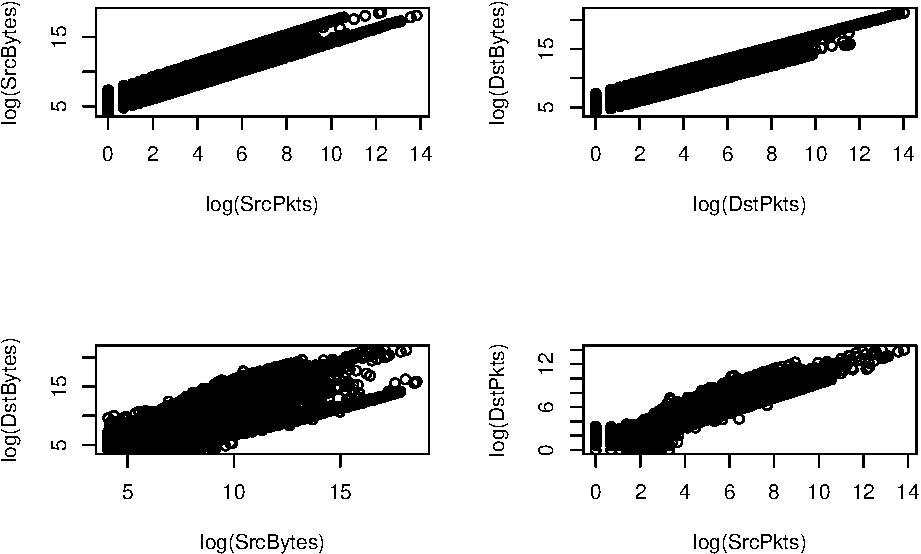
\includegraphics{thesis_files/figure-latex/unnamed-chunk-17-2.pdf}

A log transformation for each of the continuous features outputs
right-skewed histograms. Skewed features may affect the results of a
kernel pca, so we consider other approaches for transformations.

\subsection{Normal Scores
Transformation}\label{normal-scores-transformation}
\begin{Shaded}
\begin{Highlighting}[]
\NormalTok{nscore =}\StringTok{ }\NormalTok{function(x) \{}
   \CommentTok{# Takes a vector of values x and calculates their normal scores. Returns }
   \CommentTok{# a list with the scores and an ordered table of original values and}
   \CommentTok{# scores, which is useful as a back-transform table. See backtr().}
   \NormalTok{nscore =}\StringTok{ }\KeywordTok{qqnorm}\NormalTok{(x, }\DataTypeTok{plot.it =} \OtherTok{FALSE}\NormalTok{)$x  }\CommentTok{# normal score }
   \NormalTok{trn.table =}\StringTok{ }\KeywordTok{data.frame}\NormalTok{(}\DataTypeTok{x=}\KeywordTok{sort}\NormalTok{(x),}\DataTypeTok{nscore=}\KeywordTok{sort}\NormalTok{(nscore))}
   \KeywordTok{return} \NormalTok{(}\KeywordTok{list}\NormalTok{(}\DataTypeTok{nscore=}\NormalTok{nscore, }\DataTypeTok{trn.table=}\NormalTok{trn.table))}
\NormalTok{\}}

\NormalTok{backtr =}\StringTok{ }\NormalTok{function(scores, nscore, }\DataTypeTok{tails=}\StringTok{'none'}\NormalTok{, }\DataTypeTok{draw=}\OtherTok{TRUE}\NormalTok{) \{}
   \CommentTok{# Given a vector of normal scores and a normal score object }
   \CommentTok{# (from nscore), the function returns a vector of back-transformed }
   \CommentTok{# values}
   \CommentTok{# 'none' : No extrapolation; more extreme score values will revert }
   \CommentTok{# to the original min and max values. }
   \CommentTok{# 'equal' : Calculate magnitude in std deviations of the scores about }
   \CommentTok{# initial data mean. Extrapolation is linear to these deviations. }
   \CommentTok{# will be based upon deviations from the mean of the original }
   \CommentTok{# hard data - possibly quite dangerous!}
   \CommentTok{# 'separate' :  This calculates a separate sd for values }
   \CommentTok{# above and below the mean.}
   \NormalTok{if(tails==}\StringTok{'separate'}\NormalTok{) \{ }
      \NormalTok{mean.x <-}\StringTok{ }\KeywordTok{mean}\NormalTok{(nscore$trn.table$x)}
      \NormalTok{small.x <-}\StringTok{ }\NormalTok{nscore$trn.table$x <}\StringTok{ }\NormalTok{mean.x}
      \NormalTok{large.x <-}\StringTok{ }\NormalTok{nscore$trn.table$x >}\StringTok{ }\NormalTok{mean.x}
      \NormalTok{small.sd <-}\StringTok{ }\KeywordTok{sqrt}\NormalTok{(}\KeywordTok{sum}\NormalTok{((nscore$trn.table$x[small.x]-mean.x)^}\DecValTok{2}\NormalTok{)/}
\StringTok{                       }\NormalTok{(}\KeywordTok{length}\NormalTok{(nscore$trn.table$x[small.x])-}\DecValTok{1}\NormalTok{))}
      \NormalTok{large.sd <-}\StringTok{ }\KeywordTok{sqrt}\NormalTok{(}\KeywordTok{sum}\NormalTok{((nscore$trn.table$x[large.x]-mean.x)^}\DecValTok{2}\NormalTok{)/}
\StringTok{                       }\NormalTok{(}\KeywordTok{length}\NormalTok{(nscore$trn.table$x[large.x])-}\DecValTok{1}\NormalTok{))}
      \NormalTok{min.x <-}\StringTok{ }\KeywordTok{mean}\NormalTok{(nscore$trn.table$x) +}\StringTok{ }\NormalTok{(}\KeywordTok{min}\NormalTok{(scores) *}\StringTok{ }\NormalTok{small.sd)}
      \NormalTok{max.x <-}\StringTok{ }\KeywordTok{mean}\NormalTok{(nscore$trn.table$x) +}\StringTok{ }\NormalTok{(}\KeywordTok{max}\NormalTok{(scores) *}\StringTok{ }\NormalTok{large.sd)}
      \CommentTok{# check to see if these values are LESS extreme than the}
      \CommentTok{# initial data - if so, use the initial data.}
      \CommentTok{#print(paste('lg.sd is:',large.sd,'max.x is:',max.x,'max nsc.x}
      \CommentTok{#     is:',max(nscore$trn.table$x)))}
      \NormalTok{if(min.x >}\StringTok{ }\KeywordTok{min}\NormalTok{(nscore$trn.table$x)) \{min.x <-}\StringTok{ }\KeywordTok{min}\NormalTok{(nscore$trn.table$x)\}}
      \NormalTok{if(max.x <}\StringTok{ }\KeywordTok{max}\NormalTok{(nscore$trn.table$x)) \{max.x <-}\StringTok{ }\KeywordTok{max}\NormalTok{(nscore$trn.table$x)\}}
   \NormalTok{\}}
   \NormalTok{if(tails==}\StringTok{'equal'}\NormalTok{) \{ }\CommentTok{# assumes symmetric distribution around the mean}
      \NormalTok{mean.x <-}\StringTok{ }\KeywordTok{mean}\NormalTok{(nscore$trn.table$x)}
      \NormalTok{sd.x <-}\StringTok{ }\KeywordTok{sd}\NormalTok{(nscore$trn.table$x)}
      \NormalTok{min.x <-}\StringTok{ }\KeywordTok{mean}\NormalTok{(nscore$trn.table$x) +}\StringTok{ }\NormalTok{(}\KeywordTok{min}\NormalTok{(scores) *}\StringTok{ }\NormalTok{sd.x)}
      \NormalTok{max.x <-}\StringTok{ }\KeywordTok{mean}\NormalTok{(nscore$trn.table$x) +}\StringTok{ }\NormalTok{(}\KeywordTok{max}\NormalTok{(scores) *}\StringTok{ }\NormalTok{sd.x)}
      \CommentTok{# check to see if these values are LESS extreme than the}
      \CommentTok{# initial data - if so, use the initial data.}
      \NormalTok{if(min.x >}\StringTok{ }\KeywordTok{min}\NormalTok{(nscore$trn.table$x)) \{min.x <-}\StringTok{ }\KeywordTok{min}\NormalTok{(nscore$trn.table$x)\}}
      \NormalTok{if(max.x <}\StringTok{ }\KeywordTok{max}\NormalTok{(nscore$trn.table$x)) \{max.x <-}\StringTok{ }\KeywordTok{max}\NormalTok{(nscore$trn.table$x)\}}
   \NormalTok{\}}
   \NormalTok{if(tails==}\StringTok{'none'}\NormalTok{) \{   }\CommentTok{# No extrapolation}
      \NormalTok{min.x <-}\StringTok{ }\KeywordTok{min}\NormalTok{(nscore$trn.table$x)}
      \NormalTok{max.x <-}\StringTok{ }\KeywordTok{max}\NormalTok{(nscore$trn.table$x)}
   \NormalTok{\}}
   \NormalTok{min.sc <-}\StringTok{ }\KeywordTok{min}\NormalTok{(scores)}
   \NormalTok{max.sc <-}\StringTok{ }\KeywordTok{max}\NormalTok{(scores)}
   \NormalTok{x <-}\StringTok{ }\KeywordTok{c}\NormalTok{(min.x, nscore$trn.table$x, max.x)}
   \NormalTok{nsc <-}\StringTok{ }\KeywordTok{c}\NormalTok{(min.sc, nscore$trn.table$nscore, max.sc)}
   
   \NormalTok{if(draw) \{}\KeywordTok{plot}\NormalTok{(nsc,x, }\DataTypeTok{main=}\StringTok{'Transform Function'}\NormalTok{)\}}
   \NormalTok{back.xf <-}\StringTok{ }\KeywordTok{approxfun}\NormalTok{(nsc,x) }\CommentTok{# Develop the back transform function}
   \NormalTok{val <-}\StringTok{ }\KeywordTok{back.xf}\NormalTok{(scores)}
   \KeywordTok{return}\NormalTok{(val)}
\NormalTok{\}}

\NormalTok{SrcBytes_norm =}\StringTok{ }\KeywordTok{nscore}\NormalTok{(SrcBytes)$nscore}
\NormalTok{SrcBytes_table =}\StringTok{ }\KeywordTok{nscore}\NormalTok{(SrcBytes)$trn.table}

\NormalTok{SrcPkts_norm =}\StringTok{ }\KeywordTok{nscore}\NormalTok{(SrcPkts)$nscore}
\NormalTok{SrcPkts_table =}\StringTok{ }\KeywordTok{nscore}\NormalTok{(SrcPkts)$trn.table}

\NormalTok{DstBytes_norm =}\StringTok{ }\KeywordTok{nscore}\NormalTok{(DstBytes)$nscore}
\NormalTok{DstBytes_table =}\StringTok{ }\KeywordTok{nscore}\NormalTok{(DstBytes)$trn.table}

\NormalTok{DstPkts_norm =}\StringTok{ }\KeywordTok{nscore}\NormalTok{(DstPkts)$nscore}
\NormalTok{DstPkts_table =}\StringTok{ }\KeywordTok{nscore}\NormalTok{(DstPkts)$trn.table}
\KeywordTok{par}\NormalTok{(}\DataTypeTok{mfrow=}\KeywordTok{c}\NormalTok{(}\DecValTok{2}\NormalTok{,}\DecValTok{2}\NormalTok{))}
\KeywordTok{hist}\NormalTok{(SrcBytes_norm); }\KeywordTok{hist}\NormalTok{(SrcPkts_norm); }\KeywordTok{hist}\NormalTok{(DstBytes_norm); }\KeywordTok{hist}\NormalTok{(DstPkts_norm)}
\end{Highlighting}
\end{Shaded}
\includegraphics{thesis_files/figure-latex/unnamed-chunk-18-1.pdf}

Finally, a normal scores transformation is applied to the dataset. The
normal scores transformation reassigns each feature value so that it
appears the overall data for that feature had arisen or been observed
from a standard normal distribution. This transformation solves the
issue of skewness-each value's histogram will now follow a standard
gaussian density plot-, but it may cause issues with other analysis
methods, particularly methods that are susceptible to ties in data.

\backmatter

\chapter*{References}\label{references}
\addcontentsline{toc}{chapter}{References}

\markboth{References}{References}

\noindent

\setlength{\parindent}{-0.20in} \setlength{\leftskip}{0.20in}
\setlength{\parskip}{8pt}

\hypertarget{refs}{}
\hypertarget{ref-angel2000}{}
Angel, Edward. 2000. \emph{Interactive Computer Graphics : A Top-down
Approach with Opengl}. Boston, MA: Addison Wesley Longman.

\hypertarget{ref-angel2001}{}
---------. 2001a. \emph{Batch-File Computer Graphics : A Bottom-up
Approach with Quicktime}. Boston, MA: Wesley Addison Longman.

\hypertarget{ref-angel2002a}{}
---------. 2001b. \emph{Test Second Book by Angel}. Boston, MA: Wesley
Addison Longman.


% Index?

\end{document}
